\documentclass[12pt]{article}
\usepackage{graphicx}
\usepackage{subcaption}
\usepackage[]{mcode}
\usepackage{mwe}
\usepackage{amsmath}
\usepackage[T1]{fontenc}


\DeclareMathOperator{\erf}{erf}
\renewcommand{\thesubsection}{\thesection.\alph{subsection}}

\begin{document}

\title{CMSC 460 - HW6}
\author{Gudjon Einar Magnusson}

\maketitle

\section{}

\subsection{Singular Matricies}

The following matrices are singular because the span of $Ax$ contains the zero vector when $x$ is not zero. That tells me that zero is an eigenvalue of $A$.

\[
\begin{bmatrix}
    2 & 4 \\
    2 & 4
\end{bmatrix} /4
\]

\[
\begin{bmatrix}
    2 & 4 \\
    -1 & -2
\end{bmatrix} /4
\]

\subsection{Complex $\lambda$}

The following matrices have complex eigenvalues because $x$ and $Ax$ never become parallel.

\[
\begin{bmatrix}
    0 & 1 \\
    -1 & 0
\end{bmatrix}
\]

\[
\begin{bmatrix}
    3 & 1 \\
    -2 & 4
\end{bmatrix} / 4
\]

\[
\begin{bmatrix}
    2 & 4 \\
    -1 & -2
\end{bmatrix} /4
\]

\subsection{Double $\lambda$}

The following matrices have repeated eigenvalues. 

\[
\begin{bmatrix}
    1 & 0 \\
    0 & 1
\end{bmatrix}
\]

\[
\begin{bmatrix}
    6 & 4 \\
    -1 & 2
\end{bmatrix} /4
\]

\section{}

\subsection{}

For my image matrix $I$ of size $540\times960\times3$, or $540\times2880$ after reshaping
\[[V, S, U] = svd(I, 0)\]
Gives me a large non-square sigma matrix, which is not what I want.
\[[V, S, U] = svd(I', 0)\]
Gives me a $540\times540$ sigma matrix.

\subsection{}

Figure \ref{fig_rank_approx} shows how my image approximated by matrices of different ranks. The original image is of rank 540 but the difference is almost undetectable down to rank 100. At rank 20 the image still readable but the quality drops quickly at ranks below that. That makes sense if we look at the log plot of the singular values in figure \ref{fig_sigma}. The first few singular values drop very quickly but then levels of somewhere around the 20th value and starts dropping slower.

\begin{figure}
    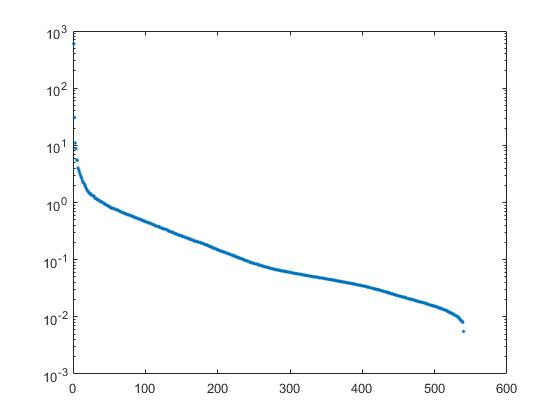
\includegraphics[width=0.6\linewidth]{plot_sigma}
    \centering
    \caption{}
    \label{fig_sigma}
\end{figure}

\begin{figure}
    \begin{subfigure}[t]{.49\textwidth}
        \centering
        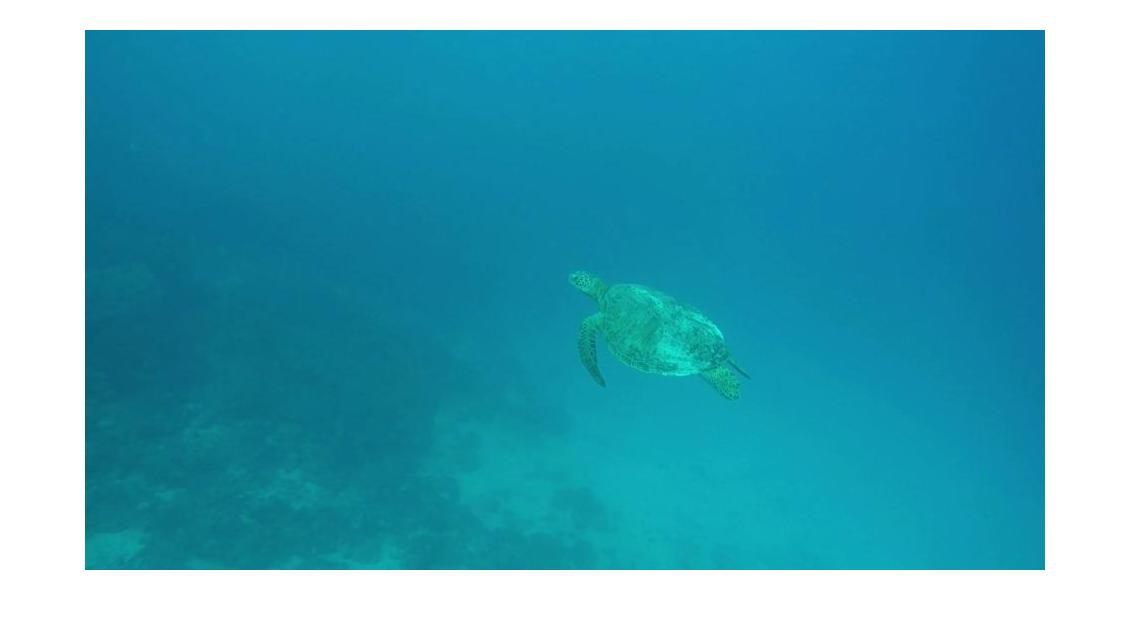
\includegraphics[width=\linewidth]{rank540}
        \caption{Original image, rank 540}
        \label{fig_rank549}
    \end{subfigure}\hfill
    \begin{subfigure}[t]{.49\textwidth}
        \centering
        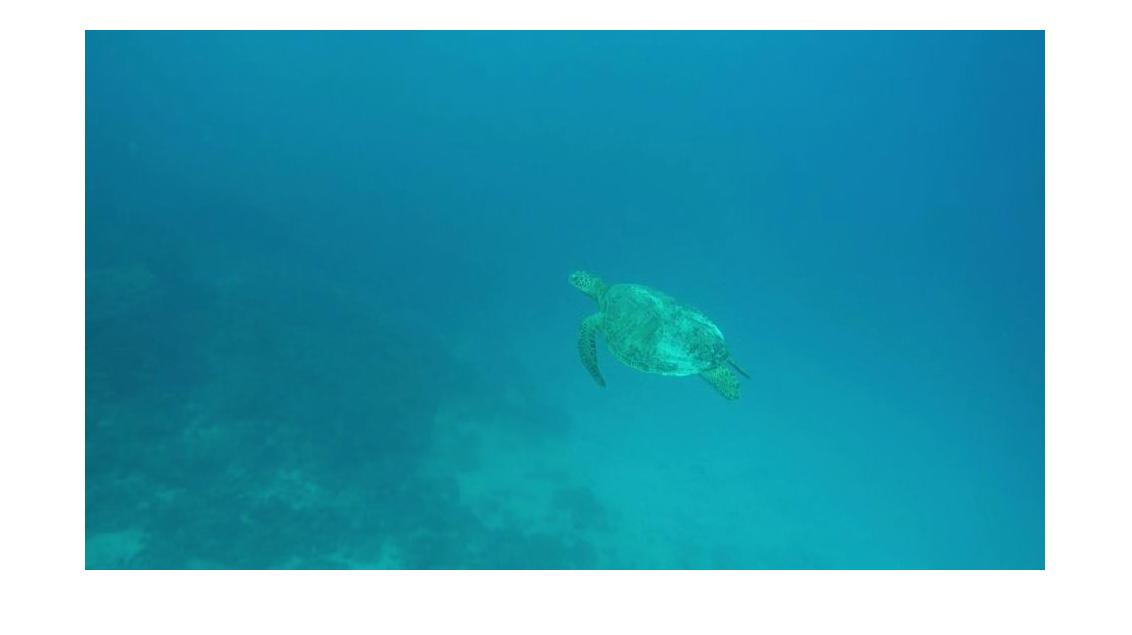
\includegraphics[width=\linewidth]{rank100}
        \caption{Rank 100 approximation}
        \label{fig_rank100}
    \end{subfigure}

    \vskip\baselineskip

    \begin{subfigure}[t]{.49\textwidth}
        \centering
        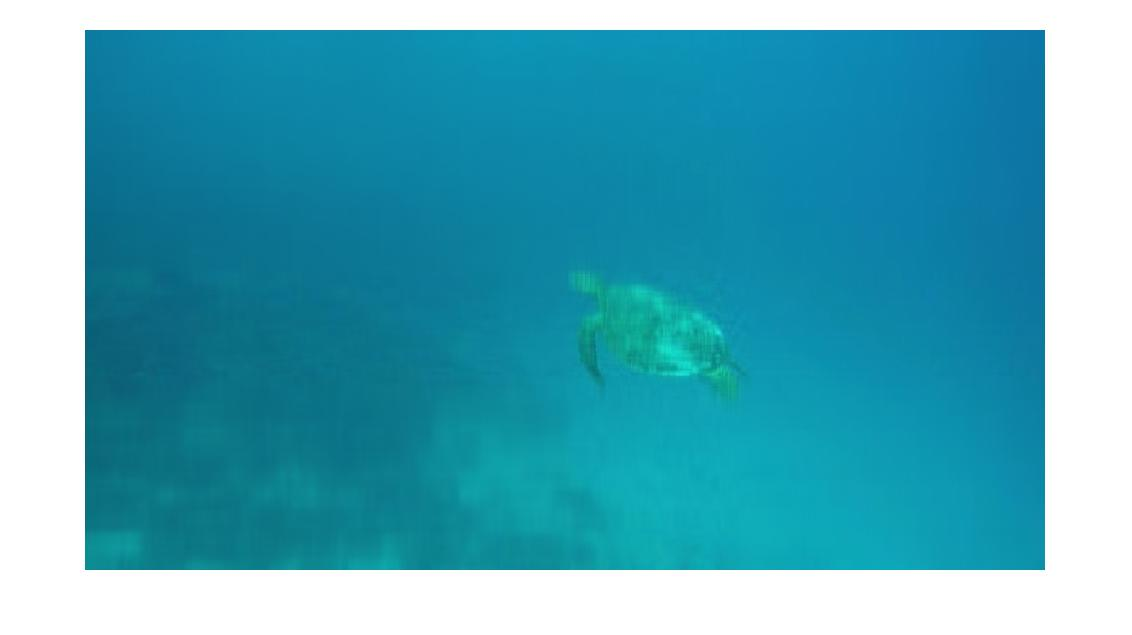
\includegraphics[width=\linewidth]{rank20}
        \caption{Rank 20 approximation}
        \label{fig_rank20}
    \end{subfigure}\hfill
    \begin{subfigure}[t]{.49\textwidth}
        \centering
        
\includegraphics[width=\linewidth]{rank1}
        \caption{Rank 1 approximation}
        \label{fig_rank1}
    \end{subfigure}
    \caption{$Rank_k$ approximation of an image}
    \label{fig_rank_approx}
\end{figure}

\end{document}